\documentclass[12pt]{article}

%%%%%%%%%%%%%%%%%%%%%%%%%%%%%%%%%%%%%%%%%%%%%%%%%%%%%%%%%%%%%%%%%%%%%%%%%%%%%%%%%%%%%%%%%%%%%%%%%%%%
% Math
\usepackage{fancyhdr} 
\usepackage{amsfonts}
\usepackage{amsmath}
\usepackage{amssymb}
\usepackage{amsthm}
%\usepackage{dsfont}

%%%%%%%%%%%%%%%%%%%%%%%%%%%%%%%%%%%%%%%%%%%%%%%%%%%%%%%%%%%%%%%%%%%%%%%%%%%%%%%%%%%%%%%%%%%%%%%%%%%%
% Macros
\usepackage{calc}

%%%%%%%%%%%%%%%%%%%%%%%%%%%%%%%%%%%%%%%%%%%%%%%%%%%%%%%%%%%%%%%%%%%%%%%%%%%%%%%%%%%%%%%%%%%%%%%%%%%%
% Commands and Custom Variables	
\newcommand{\problem}[1]{\hspace{-4 ex} \large \textbf{Problem #1} }
\let\oldemptyset\emptyset
\let\emptyset\varnothing
\newcommand{\norm}[1]{\left\lVert#1\right\rVert}
\newcommand{\sint}{\text{s}\kern-5pt\int}
\newcommand{\powerset}{\mathcal{P}}
\renewenvironment{proof}{\hspace{-4 ex} \emph{Proof}:}{\qed}
\newcommand{\RR}{\mathbb{R}}
\newcommand{\NN}{\mathbb{N}}
\newcommand{\QQ}{\mathbb{Q}}
\newcommand{\ZZ}{\mathbb{Z}}
\newcommand{\CC}{\mathbb{C}}
\renewcommand{\Re}{\operatorname{Re}}
\renewcommand{\Im}{\operatorname{Im}}


%%%%%%%%%%%%%%%%%%%%%%%%%%%%%%%%%%%%%%%%%%%%%%%%%%%%%%%%%%%%%%%%%%%%%%%%%%%%%%%%%%%%%%%%%%%%%%%%%%%%
%page
\usepackage[margin=1in]{geometry}
\usepackage{setspace}
%\doublespacing
\allowdisplaybreaks
\pagestyle{fancy}
\fancyhf{}
\rhead{Shaw \space \thepage}
\setlength\parindent{0pt}

%%%%%%%%%%%%%%%%%%%%%%%%%%%%%%%%%%%%%%%%%%%%%%%%%%%%%%%%%%%%%%%%%%%%%%%%%%%%%%%%%%%%%%%%%%%%%%%%%%%%
%Code
\usepackage{listings}
\usepackage{courier}
\lstset{
	language=Python,
	showstringspaces=false,
	formfeed=newpage,
	tabsize=4,
	commentstyle=\itshape,
	basicstyle=\ttfamily,
}

%%%%%%%%%%%%%%%%%%%%%%%%%%%%%%%%%%%%%%%%%%%%%%%%%%%%%%%%%%%%%%%%%%%%%%%%%%%%%%%%%%%%%%%%%%%%%%%%%%%%
%Images
\usepackage{graphicx}
\graphicspath{ {images/} }
\usepackage{float}

%tikz
\usepackage[utf8]{inputenc}
\usepackage{pgfplots}
\usepgfplotslibrary{groupplots}

%%%%%%%%%%%%%%%%%%%%%%%%%%%%%%%%%%%%%%%%%%%%%%%%%%%%%%%%%%%%%%%%%%%%%%%%%%%%%%%%%%%%%%%%%%%%%%%%%%%%
%Hyperlinks
%\usepackage{hyperref}
%\hypersetup{
%	colorlinks=true,
%	linkcolor=blue,
%	filecolor=magenta,      
%	urlcolor=cyan,
%}

\begin{document}
	\thispagestyle{empty}
	
	\begin{flushright}
		Sage Shaw \\
		m537 - Spring 2018 \\
		\today
	\end{flushright}
	
{\large \textbf{Take-home Project 2}}\bigbreak

Consider a heat conducting rectangle 
$$
	R = \{(x,y) \in \RR: \phantom{==} 0 \leq x \leq L, \phantom{==} 0 \leq Y \leq K \}
$$
($L$ and $K$ are positive constants) and its equilibrium temperature $u(x,y)$ with the following values prescribed on the boundaries
\begin{align*}
u(x,0) & = f_1(x), & u(x,K) & = f_2(x), & 0 \leq & x \leq L \\
u(0,y) & = g_3(y), & u(L,y) & = g_4(y), & 0 \leq & y \leq K 
\end{align*}
where $f_1,f_2, g_1$ and $g_2$ are given continuous functions. In Cartesian coordinates the temperature satisfies the equation
\begin{align}
	\frac{\partial^2 u}{\partial x^2}(x,y) + \frac{\partial^2 u}{\partial y^2}(x,y) = 0 \label{pde}
\end{align}
for $(x,y) \in \RR$. 

\problem{1. } Show that 
$$
u(x,y) = u_1(x,y) + u_2(x,y) + u_3(x,y) + u_4(x,y),
$$
where each $u_1, u_2, u_3, u_4$ satisfy (\ref{pde}) and the following boundary conditions
\begin{align*}
	u_1(x,0) & = f_1(x) &  u_1(x,K) & = 0 & u_1(0,y) &= 0 & u_1(L,y)&= 0 \\
	u_2(x,0) & = 0 &  u_2(x,K) & = f_2(x) & u_2(0,y) &= 0 & u_2(L,y)&= 0 \\
	u_3(x,0) & = 0 &  u_3(x,K) & = 0 & u_3(0,y) &= g_3(y) & u_3(L,y)&= 0 \\
	u_4(x,0) & = 0 &  u_4(x,K) & = 0 & u_4(0,y) &= 0 & u_4(L,y)&=  g_4(y) \\
	&& 0 & \leq x \leq L &  0 & \leq y \leq K &&
\end{align*}
is a solution. \bigbreak

Clearly
\begin{align*}
	& \frac{\partial^2 u}{\partial x^2}(x,y) + \frac{\partial^2 u}{\partial y^2}(x,y) \\
	& = \left( \frac{\partial^2 u_1}{\partial x^2}(x,y) + \frac{\partial^2 u_2}{\partial x^2}(x,y) 
	+ \frac{\partial^2 u_3}{\partial x^2}(x,y) + \frac{\partial^2 u_4}{\partial x^2}(x,y) \right) + \\
	& \phantom{==} \left( \frac{\partial^2 u_1}{\partial y^2}(x,y) + \frac{\partial^2 u_2}{\partial y^2}(x,y)
	+ \frac{\partial^2 u_3}{\partial y^2}(x,y) + \frac{\partial^2 u_4}{\partial y^2}(x,y) \right) \\
	& = \left( \frac{\partial^2 u_1}{\partial x^2}(x,y) + \frac{\partial^2 u_1}{\partial y^2}(x,y) \right) + 
	\left( \frac{\partial^2 u_2}{\partial x^2}(x,y) + \frac{\partial^2 u_2}{\partial y^2}(x,y) \right) + \\
	&\phantom{==} \left( \frac{\partial^2 u_3}{\partial x^2}(x,y) + \frac{\partial^2 u_3}{\partial y^2}(x,y) \right) +
	\left( \frac{\partial^2 u_4}{\partial x^2}(x,y) + \frac{\partial^2 u_4}{\partial y^2}(x,y) \right) \\
	& = 0
\end{align*}
Also for $ 0 \leq x \leq L$ and $0 \leq y \leq K$ we have that
\begin{align*}
	u(x,0) & = u_1(x,0) + u_2(x,0) + u_3(x,0) + u_4(x,0) \\
	& = f_1(x) + 0 + 0 + 0 \\
	& = f_1(x) \\
	u(x,K) & = u_1(x,K) + u_2(x,K) + u_3(x,K) + u_4(x,K) \\
	& = 0 + f_2(x) + 0 + 0 \\
	& = f_2(x) \\
	u(0,y) & = u_1(0,y) + u_2(0,y) + u_3(0,y) + u_4(0,y) \\
	& = 0 + 0 + g_3(y) + 0 \\
	& = g_3(y) \\
	u(L,y) & = u_1(L,y) + u_2(L,y) + u_3(L,y) + u_4(L,y) \\
	& = 0 + 0 + 0 + g_4(y) \\
	& = g_4(y)
\end{align*}

Thus $u$ is a solution of our PDE that satisfies all four prescribed boundary conditions. \bigbreak

\problem{2. } Let $f_2(x)=0, g_3(y)=0$ and $g_4(y)=0$. Determine $X(x)$ and $Y(y)$ such that
$$
u_1(x,y) = X(x)Y(y)
$$
\bigbreak

If two such functions existed, then we would have
\begin{align*}
	0 & = \frac{\partial^2 u_1}{\partial x^2}(x,y) + \frac{\partial^2 u_1}{\partial y^2}(x,y) \\
	& = X^{\prime\prime}Y + XY^{\prime\prime} \\
	\frac{X{\prime\prime}}{X} & = - \frac{Y^{\prime\prime}}{Y}  = -\lambda
\end{align*}
for some constant $\lambda$. This last step is because we have two functions of independent variables that are always equal. From this we get
\begin{align}
	X^{\prime\prime} + \lambda X & = 0 \label{xode} \\
	Y^{\prime\prime} - \lambda Y & = 0 \label{yode}
\end{align}
From the boundary conditions we get
\begin{align}
	0 & = u_1(x,K) = X(x)Y(K) & \implies && Y(K) &= 0 \label{yupper}\\
	0 & = u_1(0,y) = X(0)Y(y) & \implies && X(0) &= 0 \label{xlower}\\
	0 & = u_1(L,y) = X(L)Y(y) & \implies && X(L) &= 0 \label{xupper} 
\end{align}

Suppose that $\lambda < 0$. Then from (\ref{xode}) we get that 
$$
X(x) = A\cosh(\sqrt{\lambda}x) + B \sinh(\sqrt{\lambda}x)
$$
Applying (\ref{xlower}) we get
\begin{align*}
0 & = X(0) \\
& = A\cosh(\sqrt{\lambda}0) + B \sinh(\sqrt{\lambda}0) \\
& = A
\end{align*}
Applying (\ref{xupper}) we get
\begin{align*}
0 & = X(L) \\
& = B \sinh(\sqrt{\lambda}L) \\
\end{align*}
Thus either $\lambda = 0$ or $B = 0$. In either case we have the trivial solution. \bigbreak

Suppose $\lambda \geq 0$. Then from (\ref{xode}) we have
$$
X(x) = A\cos(\sqrt{\lambda}x) + B \sin(\sqrt{\lambda}x)
$$
Applying (\ref{xlower}) we get
\begin{align*}
0 & = X(0) \\
& = A\cos(\sqrt{\lambda}0) + B \sin(\sqrt{\lambda}0) \\
& = A
\end{align*}
Applying (\ref{xupper}) we get
\begin{align*}
0 & = X(L) \\
& = B \sin(\sqrt{\lambda}L) \\
\end{align*}
Thus either $B=0$ in which case we would have the trivial solution, or $\lambda = \left( \frac{n\pi}{L} \right)^2$ for $n \in \NN$. We now have infinitely many linearly independent solutions to (\ref{xode})
$$
X_n(x) = \sin \left( \frac{n\pi}{L}x \right)
$$
Also we can see that
$$
Y(y) = A\cosh(-\sqrt{\lambda}(K-y)) + B \sinh(-\sqrt{\lambda}(K-y))
$$
is a general solution to (\ref{yode}). Applying (\ref{yupper}) we get
\begin{align*}
	0 & = Y(K) \\
	& = A\cosh(-\sqrt{\lambda}(K-K)) + B \sinh(-\sqrt{\lambda}(K-K)) \\
	& = A
\end{align*}
Thus our general solutions to (\ref{yode}) are of the form
$$
Y_n(y) = \sinh \left( -\frac{n\pi}{L}(K-y) \right)
$$
and general solutions to our PDE in this case are
$$
u_n(x,y) = \sin \left( \frac{n\pi}{L}x \right) \sinh \left( \frac{n\pi}{L}(y - K) \right)
$$

\problem{3. } Let $f_1(x) = x(1-x), f_2(x) = 0, g_3(y)=0, g_4(y)=0, L=1$ and $K=2$. Then 
$$
u_n(x,y) = \sin( n\pi x ) \sinh( n\pi(y - 2) )
$$
are solutions to our PDE and a general solution is given by
$$
u(x,y) = \sum\limits_{n=1}^\infty B_n\sin( n\pi x ) \sinh( n\pi(y - 2))
$$
Applying our final boundary condition we get
\begin{align*}
f_1(x) & = u(x,0) \\
& = \sum\limits_{n=1}^\infty B_n \sin( n\pi x ) \sinh( -2 n\pi)
\end{align*}
From our study of Fourier Series we can conclude that
\begin{align*}
	B_n \sinh( -2 n\pi) & = 2 \int_0^1 f_1(x) \sin( n\pi x ) dx \\
	B_n & = \frac{2}{\sinh( -2 n\pi)} \int_0^1 f_1(x) \sin( n\pi x ) dx \\
	& = \frac{2}{\sinh( -2 n\pi)} \frac{-\pi n \sin(\pi n) - 2 \cos(\pi n) + 2}{\pi^3 n^3} \text{\ \ (from Wolfram Alpha)} \\
	& = \frac{2}{\sinh( -2 n\pi)} \frac{- 2 (-1)^n + 2}{\pi^3 n^3} \\
	& = \frac{4 (-1)^n - 4 }{\sinh( 2 n\pi) \pi^3 n^3} \\
\end{align*}

Thus our solution is
$$
u(x,y) = \sum\limits_{n=1}^\infty B_n\sin( n\pi x ) \sinh( n\pi(y - 2))
$$
where $B_n$ is given by
$$
B_n = \begin{cases}
	\frac{-8}{\sinh( 2 n\pi) \pi^3 n^3} & n \text{ odd} \\
	0 & n \text{ even}
\end{cases}
$$

\problem{4. } Figure \ref{fig1} shows this solution approximated with the tenth partial sum. It looks like a very reasonable solution to the problem. This makes sense since $B_n$ decreases sharply as $n$ increases. For example $B_9 = -1.955\times 10^{-28}$, a very small term indeed!

\begin{figure}[H]
	\caption{$u$ approximated with $n=10$ terms}
	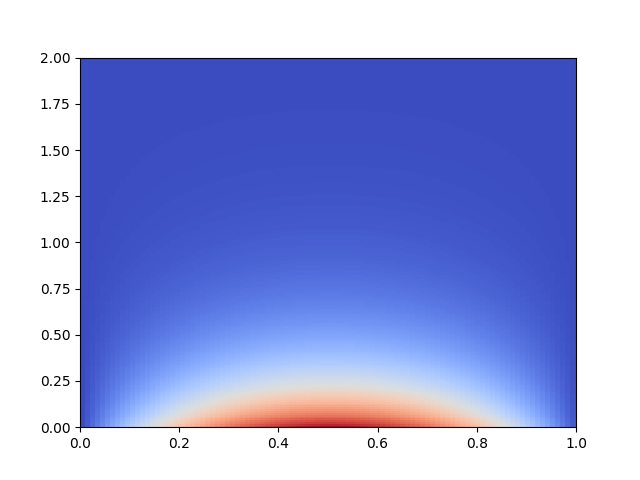
\includegraphics[width=1\textwidth]{tk02_figure1_png}
	\label{fig1}
	\centering
\end{figure}

\end{document}
